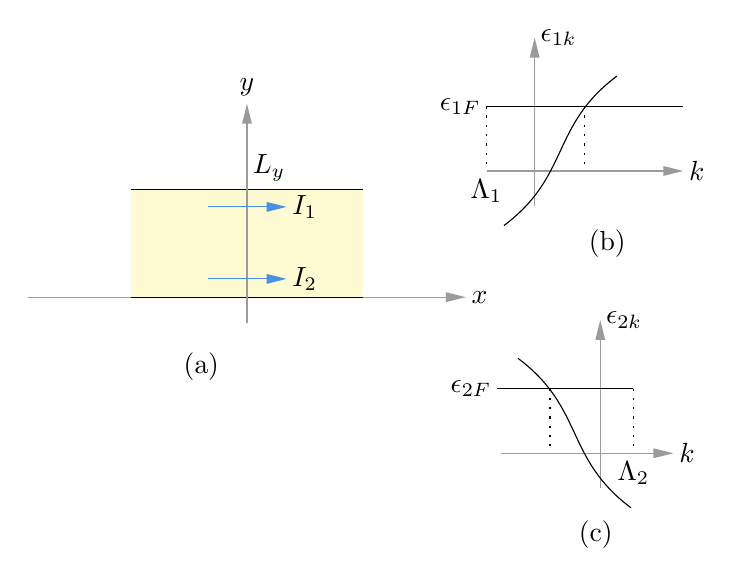
\begin{tikzpicture}[x=0.75pt,y=0.75pt,yscale=-0.8,xscale=0.8]
    %uncomment if require: \path (0,338); %set diagram left start at 0, and has height of 338
    
    %Shape: Rectangle [id:dp40795066059982865] 
    \draw  [draw opacity=0][fill={rgb, 255:red, 248; green, 231; blue, 28 }  ,fill opacity=0.2 ] (111,110) -- (250.5,110) -- (250.5,175) -- (111,175) -- cycle ;
    %Straight Lines [id:da36690056790944925] 
    \draw [color={rgb, 255:red, 155; green, 155; blue, 155 }  ,draw opacity=1 ]   (49,175) -- (310.5,175) ;
    \draw [shift={(312.5,175)}, rotate = 180] [fill={rgb, 255:red, 155; green, 155; blue, 155 }  ,fill opacity=1 ][line width=0.08]  [draw opacity=0] (12,-3) -- (0,0) -- (12,3) -- cycle    ;
    %Straight Lines [id:da6580792285138533] 
    \draw    (111,110) -- (250.5,110) ;
    %Straight Lines [id:da2884770612696377] 
    \draw    (111,175) -- (250.5,175) ;
    %Straight Lines [id:da7254005793637499] 
    \draw [color={rgb, 255:red, 155; green, 155; blue, 155 }  ,draw opacity=1 ]   (180.75,190.74) -- (180.75,60.52) ;
    \draw [shift={(180.75,58.52)}, rotate = 90] [fill={rgb, 255:red, 155; green, 155; blue, 155 }  ,fill opacity=1 ][line width=0.08]  [draw opacity=0] (12,-3) -- (0,0) -- (12,3) -- cycle    ;
    %Straight Lines [id:da5230554548972957] 
    \draw [color={rgb, 255:red, 74; green, 144; blue, 226 }  ,draw opacity=1 ][fill={rgb, 255:red, 74; green, 144; blue, 226 }  ,fill opacity=1 ]   (157,120.63) -- (202.5,120.63) ;
    \draw [shift={(204.5,120.63)}, rotate = 180] [fill={rgb, 255:red, 74; green, 144; blue, 226 }  ,fill opacity=1 ][line width=0.08]  [draw opacity=0] (12,-3) -- (0,0) -- (12,3) -- cycle    ;
    %Straight Lines [id:da26319630873635913] 
    \draw [color={rgb, 255:red, 74; green, 144; blue, 226 }  ,draw opacity=1 ][fill={rgb, 255:red, 74; green, 144; blue, 226 }  ,fill opacity=1 ]   (157,164) -- (202.5,164) ;
    \draw [shift={(204.5,164)}, rotate = 180] [fill={rgb, 255:red, 74; green, 144; blue, 226 }  ,fill opacity=1 ][line width=0.08]  [draw opacity=0] (12,-3) -- (0,0) -- (12,3) -- cycle    ;
    %Straight Lines [id:da6574829504537725] 
    \draw [color={rgb, 255:red, 155; green, 155; blue, 155 }  ,draw opacity=1 ]   (325,99) -- (441.5,99) ;
    \draw [shift={(443.5,99)}, rotate = 180] [fill={rgb, 255:red, 155; green, 155; blue, 155 }  ,fill opacity=1 ][line width=0.08]  [draw opacity=0] (12,-3) -- (0,0) -- (12,3) -- cycle    ;
    %Straight Lines [id:da9847646340319416] 
    \draw [color={rgb, 255:red, 155; green, 155; blue, 155 }  ,draw opacity=1 ]   (354,120) -- (354,20.78) ;
    \draw [shift={(354,18.78)}, rotate = 90] [fill={rgb, 255:red, 155; green, 155; blue, 155 }  ,fill opacity=1 ][line width=0.08]  [draw opacity=0] (12,-3) -- (0,0) -- (12,3) -- cycle    ;
    %Curve Lines [id:da6788189381158845] 
    \draw    (335.5,131.85) .. controls (375.5,101.85) and (363.5,71.85) .. (403.5,41.85) ;
    %Straight Lines [id:da9121250772726961] 
    \draw    (325,60) -- (443.5,60) ;
    %Straight Lines [id:da3059306191704432] 
    \draw  [dash pattern={on 0.84pt off 2.51pt}]  (325,60) -- (325,99) ;
    %Straight Lines [id:da5759142882874566] 
    \draw  [dash pattern={on 0.84pt off 2.51pt}]  (384.25,60) -- (384.25,99) ;
    
    %Straight Lines [id:da40262000917674734] 
    \draw [color={rgb, 255:red, 155; green, 155; blue, 155 }  ,draw opacity=1 ]   (435.5,269) -- (333.5,269) ;
    \draw [shift={(437.5,269)}, rotate = 180] [fill={rgb, 255:red, 155; green, 155; blue, 155 }  ,fill opacity=1 ][line width=0.08]  [draw opacity=0] (12,-3) -- (0,0) -- (12,3) -- cycle    ;
    %Straight Lines [id:da7191872218882651] 
    \draw [color={rgb, 255:red, 155; green, 155; blue, 155 }  ,draw opacity=1 ]   (393.5,290) -- (393.5,190.78) ;
    \draw [shift={(393.5,188.78)}, rotate = 90] [fill={rgb, 255:red, 155; green, 155; blue, 155 }  ,fill opacity=1 ][line width=0.08]  [draw opacity=0] (12,-3) -- (0,0) -- (12,3) -- cycle    ;
    %Curve Lines [id:da8130155872478908] 
    \draw    (412,301.85) .. controls (372,271.85) and (384,241.85) .. (344,211.85) ;
    %Straight Lines [id:da4797731726124772] 
    \draw    (413.5,230) -- (331.5,230) ;
    %Straight Lines [id:da508293409330584] 
    \draw  [dash pattern={on 0.84pt off 2.51pt}]  (363.25,230) -- (363.25,269) ;
    %Straight Lines [id:da8016612780997885] 
    \draw  [dash pattern={on 0.84pt off 2.51pt}]  (413.5,230) -- (413.5,269) ;
    
    
    % Text Node
    \draw (182.75,106.6) node [anchor=south west] [inner sep=0.75pt]    {$L_{y}$};
    % Text Node
    \draw (314.5,175) node [anchor=west] [inner sep=0.75pt]    {$x$};
    % Text Node
    \draw (180.75,55.12) node [anchor=south] [inner sep=0.75pt]    {$y$};
    % Text Node
    \draw (206.5,120.63) node [anchor=west] [inner sep=0.75pt]    {$I_{1}$};
    % Text Node
    \draw (206.5,164) node [anchor=west] [inner sep=0.75pt]    {$I_{2}$};
    % Text Node
    \draw (439.5,269) node [anchor=west] [inner sep=0.75pt]    {$k$};
    % Text Node
    \draw (395.5,188.78) node [anchor=west] [inner sep=0.75pt]    {$\epsilon _{2k}$};
    % Text Node
    \draw (413.5,272.4) node [anchor=north] [inner sep=0.75pt]    {$\Lambda _{2}$};
    % Text Node
    \draw (329.5,230) node [anchor=east] [inner sep=0.75pt]   [align=left] {$\displaystyle \epsilon _{\text{2F}}$};
    % Text Node
    \draw (445.5,99) node [anchor=west] [inner sep=0.75pt]    {$k$};
    % Text Node
    \draw (356,18.78) node [anchor=west] [inner sep=0.75pt]    {$\epsilon _{1k}$};
    % Text Node
    \draw (325,102.4) node [anchor=north] [inner sep=0.75pt]    {$\Lambda _{1}$};
    % Text Node
    \draw (323,60) node [anchor=east] [inner sep=0.75pt]   [align=left] {$\displaystyle \epsilon _{1\text{F}}$};
    % Text Node
    \draw (141,207) node [anchor=north west][inner sep=0.75pt]   [align=left] {(a)};
    % Text Node
    \draw (385,133) node [anchor=north west][inner sep=0.75pt]   [align=left] {(b)};
    % Text Node
    \draw (379,308) node [anchor=north west][inner sep=0.75pt]   [align=left] {(c)};
    
    
    \end{tikzpicture}
    